\documentclass[../main.tex]{subfiles}
\graphicspath{{img},{img/ink},{ink}}

\begin{document}

\begin{tcolorbox}[
    width=\textwidth,
    height=\textheight,
    title=Versuch: Auf- und Entladekurve eines Kondensators,
    fonttitle=\Large,
    before title=\vspace{0.2cm}, after title=\vspace{0.2cm},
    colback=white,
    title filled=true, 
    colbacktitle=mygray,
    colframe=black,
    coltitle=black,
]
    
    \vspace{0.2cm}
\textbf{Klassenstufe}: 9/10

    \vspace{0.5cm}
    
    \textbf{Fachlicher Bezug}: Kondensator, Zeitkonstante, Spannungs- und Strommessung 
    
    \vspace{0.5cm}
    
    \textbf{Material}: Mobile-CASSY + 2 Sensorstecker, iPad + CASSY-App, Netzgerät 30 V, Kondensator $C=0.1 \, \text{F}$, Widerstand $R = 47 \, \Omega$, Schalter, Experimentierkabel

    \vspace{0.5cm}
        \begin{minipage}[c]{0.5\textwidth}
            \centering
            \includegraphics[width=0.85\textwidth]{img/versuchsaufbau}
        \end{minipage}
        \begin{minipage}[c]{0.5\textwidth}
            \vspace{-0.3cm}
            \begin{center}
                \begin{circuitikz} 
                \ctikzset{
                    bipoles/capacitor/width/.initial=.1,
                    european resistors
                }
                \draw   (0,0) node[spdt] (s) {}
                % middle part
                (s.in) to [short] (-1,0) coordinate (cr)
                %(cr) node[circ] {}
                (cr) to [C, l_={$C$}] (-2,0) coordinate (cl)
                %(cl) node[circ] {}
                % voltage measurement
                (cr) to [short] (-1,-1.4) coordinate (voltmeter_right)
                (cl) to [short] (-2,-1.4) coordinate (voltmeter_left)
                (voltmeter_left) to [voltmeter] (voltmeter_right)
                % current measurement
                (cl) to [R={$R$}] (-4,0) coordinate (rl)
                (rl) to [ammeter,mirror,invert] (-5.5,0) coordinate (al)
                %bottom part
                (al) to [short] (-5.5,-2) coordinate (al_down)
                (s.out 2) to [short] (s.out 2|-0,-2) coordinate (s_out_2_down)
                (s_out_2_down) to [short] (al_down)
                %top part
                (al) to [short] (-5.5,1.5) coordinate (al_up)
                (s.out 1) to [short] (s.out 1|-0,1.5) coordinate (s_out_1_up)
                (s_out_1_up) to [battery1, xshift=-5mm] (al_up)
                ;
                \node at (-2.3,1.9) {$U$};
                \draw (al_down) ++ (0,0.3) node[ground]{}; 
            \end{circuitikz}
            \end{center}
            
        \end{minipage}
    
    \vspace{0.5cm}
    \textbf{Aufbau}: Das Experiment besteht aus Lade- und Entladestromkreis. Ein Schalter ermöglicht einen Wechsel. Steckplätze am Mobile-CASSY messen die Stromstärke und die Spannung. Die Messung der Stromstärke (in Reihe) muss im Lade- und Entladestromkreis möglich sein. Die Spannungsmessung erfolgt parallel zum Kondensator. Das Mobile-CASSY stellt einen Wlan-Access-Point zur Verfügung. Um eine Verbindung mit dem iPad herzustellen, verbindet man sich mit dem Access-Point und startet die CASSY-App. 
    
    \vspace{0.5cm} 
    \begin{minipage}[]{0.74\textwidth}
        \textbf{Durchführung}: Der Versuch startet mit geschlossenem Entladestromkreis. Im Ladestromkreis liegt eine Spannung $U=5$ V an. Die Messwertaufnahme in der CASSY-App wird gestartet. Lade-und Entladevorgang werden aufgezeichnet. 

        \vspace{0.5cm}
    \textbf{Ergebnis}: Man erhält die dargestellten Lade-und Entladekurven. Die schwarze Kurve zeigt den Verlauf der gespeicherten Spannung $U_C(t)$ im Kondensator. Die rote Kurve zeigt die Stromstärke $I(t)$. Beim Aufladen gilt dabei
\begin{align*}
    U_C(t) = U \cdot \left( 1-e^{-\frac{t}{\tau}}\right ) \qquad I(t)=I_0 \cdot e^{-\frac{t}{\tau}} \quad \text{mit} \,\, \tau = R \cdot C
\end{align*}
    
    
\end{minipage}
\hspace{0.05cm}    
\begin{minipage}[]{0.24\textwidth}
        \vspace{-0.2cm}
        \begin{center}
            \includegraphics[width=1\textwidth]{img/cassy}
        \end{center}
    \end{minipage}
  
    \vspace{0.5cm}
    \textbf{Didaktische Bemerkungen}: Beim Entladevorgang wird eine Umkehr in der Stromrichtung beobachtet. Vor Versuchsbeginn können dazu Hypothesen aufgestellt werden.      
    
    \vspace{0.5cm}
    \textbf{Bemerkungen}: Die Zeitkonstante $\tau=R \cdot C$ entspricht der Zeit, bei der die Kondensatorspannung auf $63 \%$ ($1-1/e$) des Endwerts angestiegen, bzw. der Ladestom auf $37 \%$ ($1/e$) abgefallen ist. \\
    Um eine möglichst hohe Abtastrate der Sensorstecker zu erreichen, ist es sinnvoll, Spannung- und Strommessung getrennt, an zwei verschiedenen Steckplätzen, vorzunehmen. Außerdem kann es bei der Verwendung der CASSY-App zu Schwierigkeiten bei der Positionierung des Koordinatensystems kommen. Hier hilft in der Regel ein kurzer Wechsel der Steckplätze.
\end{tcolorbox}


\end{document}
